\subsection{Execution stage}
The execution stage contains the blocks that carry out the calculations, including the ALU, the Forwarding Unit, the PC incrementer and some useful units to manage data flows. Each operation lasts one clock cycle so there are no pipeline stages within the stage but only before and after. In figure \todo{Insert figure} all the blocks and the data path can be seen.\\
The ALU has two inputs which are partly managed by the instruction decoded by the CU and partly by the forwarding unit in case data dependencies are present. In the case of non-hazardous operation, port "A" of the ALU contains data "A" from the register file or the non-incremented PC, while port "B" contains data from port "B" of the register file or the Immediate from the instruction. In this way all instructions can be handled without ever having an overlap in the port request. On the other hand, when data dependencies are present, these data are ignored and bypassed by the forwarding unit's decision in order to insert the correct data. The management of the branch instruction requires the evaluation of equality between two data and is carried out by a separate unit from the ALU as it is busy in calculating the jump address, i.e. the sum between the PC and the displacement present in the Immediate. Some units are analysed in detail in the following subsections.

\subsubsection{ALU}

\subsubsection{Forwarding Unit}
The forwarding unit is responsible for resolving all data dependencies between the Execute stage and the other pipeline stages. In particular, it looks for situations in which the source register of the current instruction coincides with the destination address of the instruction processed one or two clock cycles earlier.
\begin{figure}[htbp]
	\centering
	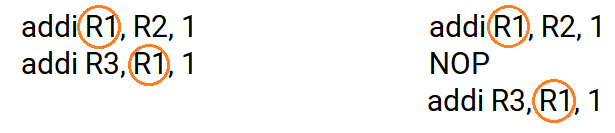
\includegraphics[width=0.5\textwidth]{sec2/images/data_dependency.png}
	\caption{Example of data dependencies solved by the forwarding unit}
	\label{fig:zero_skipping}
\end{figure}
\\In the first case, the data is taken from the output register of the ALU, instead of the register file. In the second case from the memory output register. In this way the data is forwarded without waiting for the correct data to be written in the register file. Each time the forwarding unit starts up, there is a benefit that corresponds to one or two clock cycles. To understand if the bits of the source and destination addresses are valid it is necessary to check that the instructions they refer to use such fields, i.e. if the instruction is of the type \textit{R, I, U, J}.\\
The forwarding unit also handles Store instructions, which write directly to memory by forwarding the data from the ALU output register or the memory output register to the data memory input.\\
Since the branch evaluation is also done on data from the register file, it requires the forwarding of data of both inputs.
